\section{Delay de Propagación - Rise Time - Fall Time}

En esta parte del artículo se propondrá medir los tiempo de propagación,
rise y fall del 74HC02. A fin de comparar resultados, primero se realizarán
mediciones en vacío y luego se repetirán utilizando el siguiente circuito:

\begin{figure}[H]
\begin{centering}
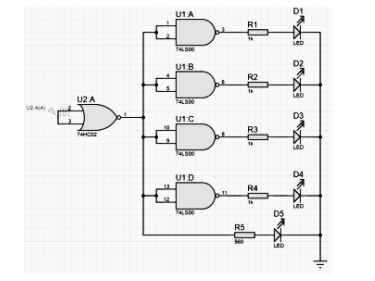
\includegraphics[scale=0.6]{circuitoAmedir.PNG}
\par\end{centering}
\begin{centering}
\caption{Circuito propuesto a medir.}
\par\end{centering}
\end{figure}


\subsection{Resultados Obtenidos}

Los resultados obtenidos fueron los siguientes:

\begin{table}[H]
\centering
\begin{tabular}{|c|c|}
\hline 
Medición en Vacío & \tabularnewline
\hline 
\hline 
Tiempo de Rise & 59 ns\tabularnewline
\hline 
Tiempo de Fall & 165 ns\tabularnewline
\hline 
Tiempo de Propagación & 15 ns\tabularnewline
\hline 
\end{tabular}\qquad
\begin{tabular}{|c|c|}
\hline 
Medición del Circuito Propuesto & \tabularnewline
\hline 
\hline 
Tiempo de Rise & 51 ns\tabularnewline
\hline 
Tiempo de Fall & 60 ns\tabularnewline
\hline 
Tiempo de Propagación & 18 ns\tabularnewline
\hline 
\end{tabular}

\caption{Mediciones - Resultados Obtenidos}

\end{table}

Estas mediciones se realizaron con una excitación de onda cuadrada
de 500 Hz de frecuencia y con una alimentación de 5 Volts.

Con respecto al tiempo de propagación con el circuito de carga, es
esperable que este sea mayor como lo indicó la medición ya que la
carga presenta una componente capacitiva que aletarga la salida medida.

Luego de realizar estas mediciones, se procedió a aumentar la frecuencia
del generador a 100 KHz y se midió la tensión de alimentación. Lo que
se observó fue que esta no resultaba ser constante. Por consiguiente,
se procedió a colocar un capacitor de $100nF$ entre los bornes de
la alimentación (entre ''Vcc'' y ''Ground'') a fin de comparar
resultados. A continuación se presentan las dos mediciones de la tensión
de alimentación (con capacitor y sin capacitor):

\begin{figure}[H]
    \centering
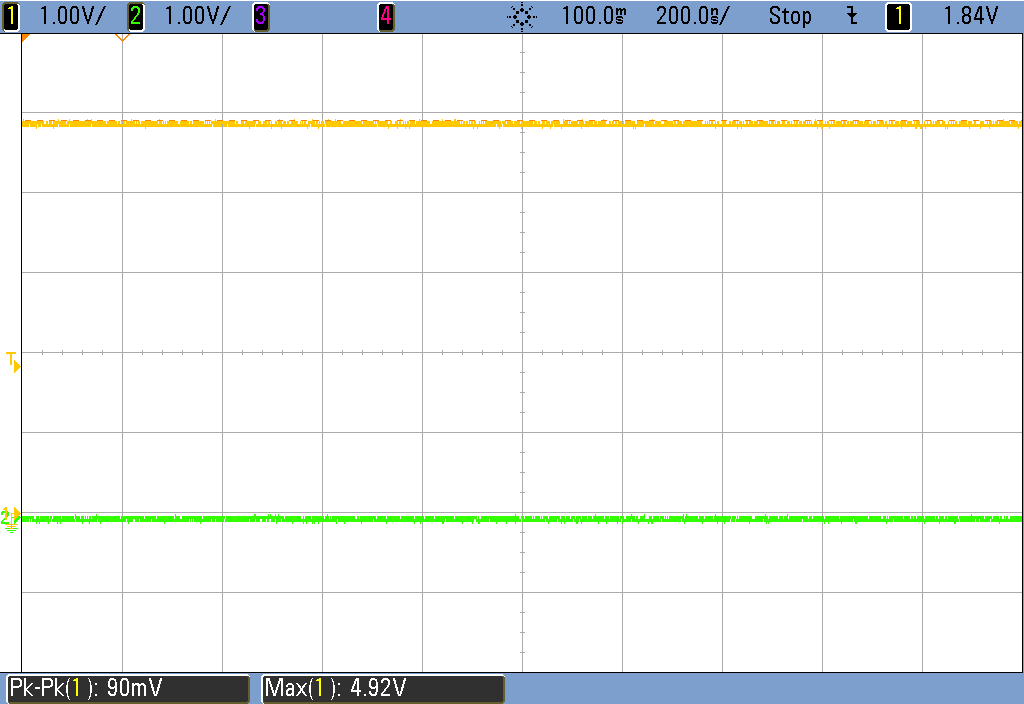
\includegraphics[scale=0.3]{AlimentacionConDesacople}
\qquad
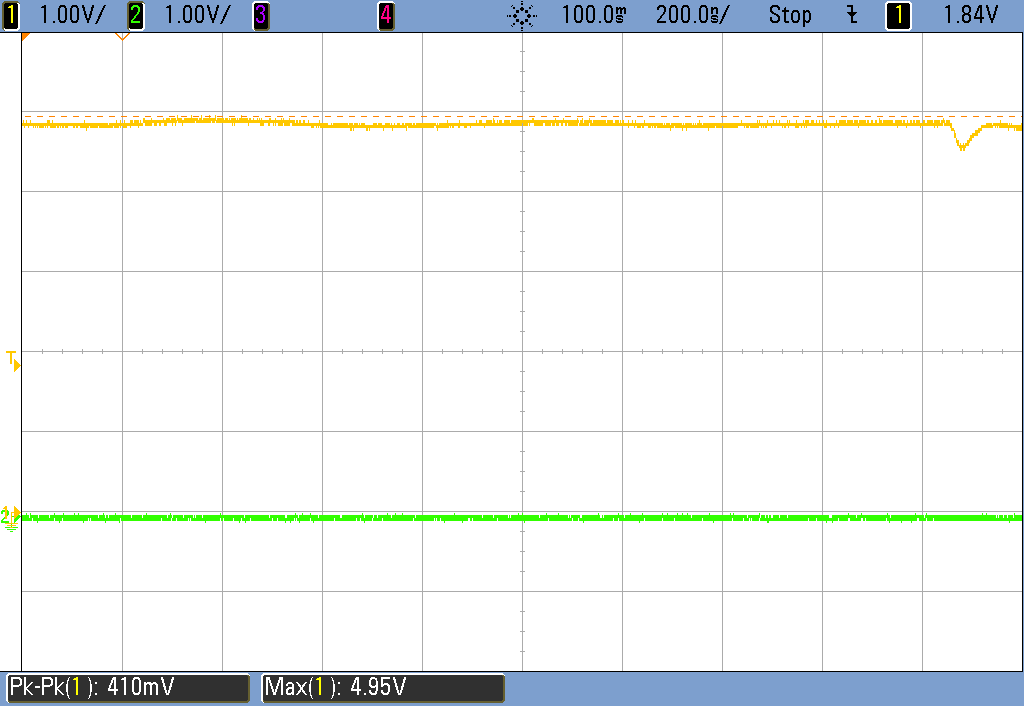
\includegraphics[scale=0.3]{AlimentacionSinDesacople}
\caption{Mediciones - Tensión de Alimentación}
\end{figure}

En la medición sin capacitor se observa un pico para el cual la tensión
de alimentación disminuye, pero que no aparece en la medición con
capacitor. Esto se puede explicar debido a que el capacitor contrarresta
las inductancias que existen debido a las conexiones físicas y además
el capacitor (si es lo suficientemente grande) es capaz de otorgar
picos de corriente que pueden requerir los transistores del integrado,
sin afectar la tensión de alimentación.

Además, al agregar el capacitor se pudo observar un cambio en la forma
de la respuesta de la 74HC02, siendo esta sub-amortiguada con sobre
pico al no colocar el capacitor, pero si se colocaba el capacitor
esta tendía a ser sobre amortiguada, sin sobre pico. A continuación
se muestran dos imágenes que plasman la diferencia de la salida de
la compuerta debida al capacitor de $100nF$:

\begin{figure}[H]
\centering
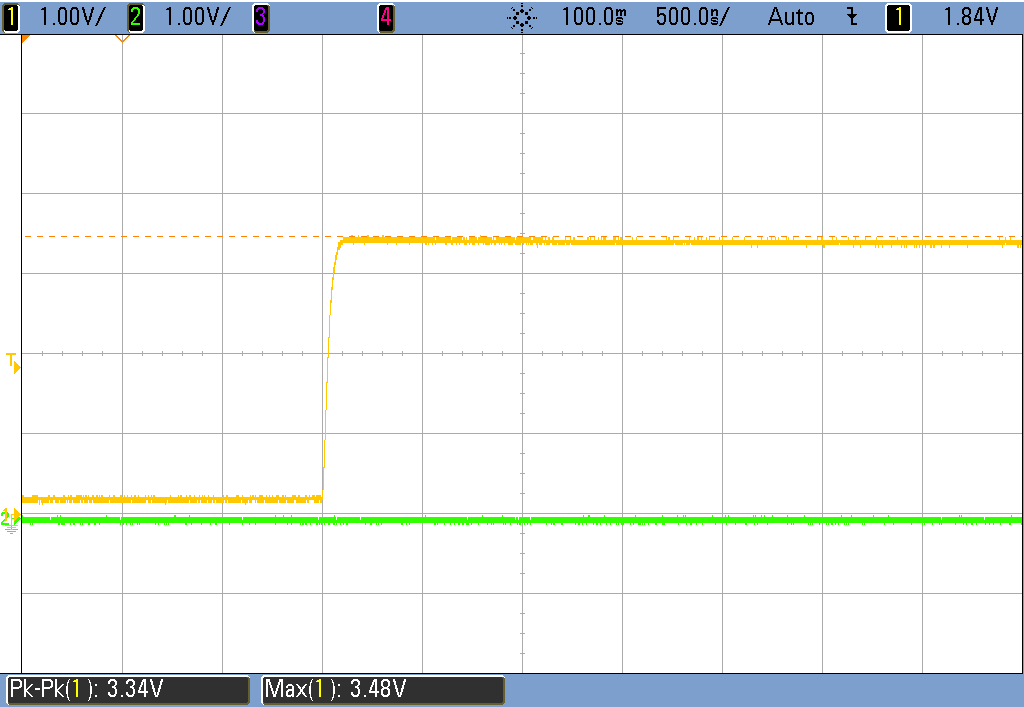
\includegraphics[scale=0.2]{SalidaDeHConDesacople}
\qquad
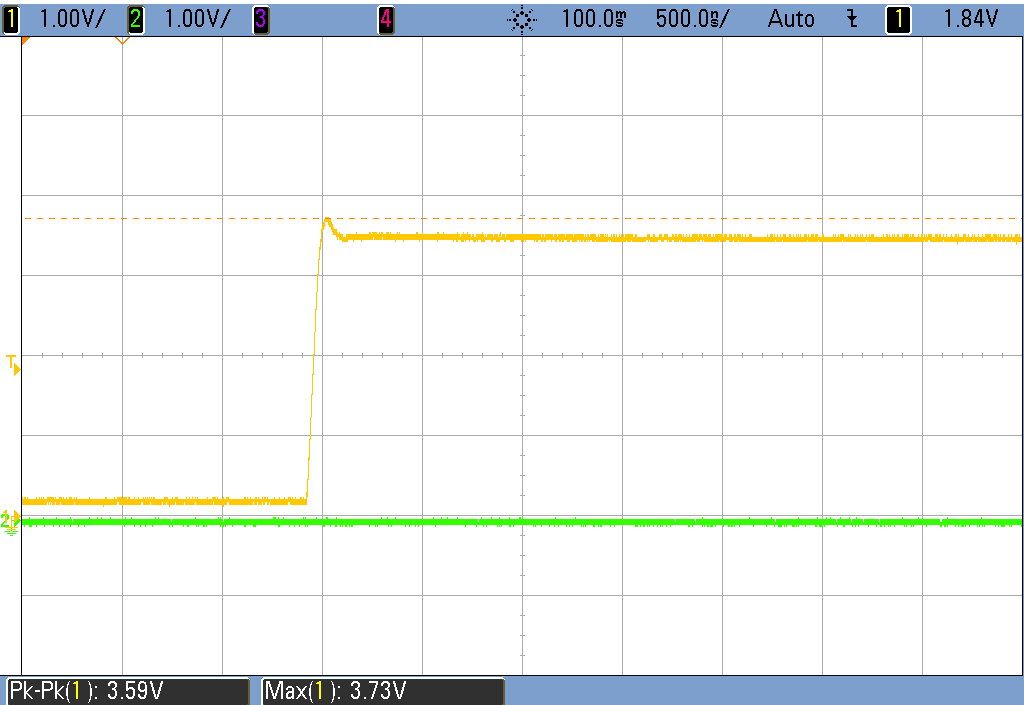
\includegraphics[scale=0.2]{SalidaDeHCSinDesacople}
\caption{Respuesta de 74HC02 según acople capacitivo.}
\end{figure}